\chapter{Fundamentação teórica}

Sobre a fundamentação teórica, o \citeonline{ftec18} diz o seguinte:

\begin{citacao}
"A fundamentação teórica consiste num levantamento sobre a temática, fornecendo uma visão geral do que já existe escrito sobre o assunto e que serve como base para a investigação prática. Entretanto, todo o texto deve ser escrito com as palavras do autor da monografia ou TCC. As citações complementam, fundamentam e justificam as ideias que estão sendo descritas."
\end{citacao}

\section{Assunto 1}

Para o \citeonline{autorx13}, esse é um exemplo de citação curta.

\lipsum[1-2]

\begin{figure}[!ht]
    \centering
    \caption{Fachada do Uniftec}
    \label{graf1}
    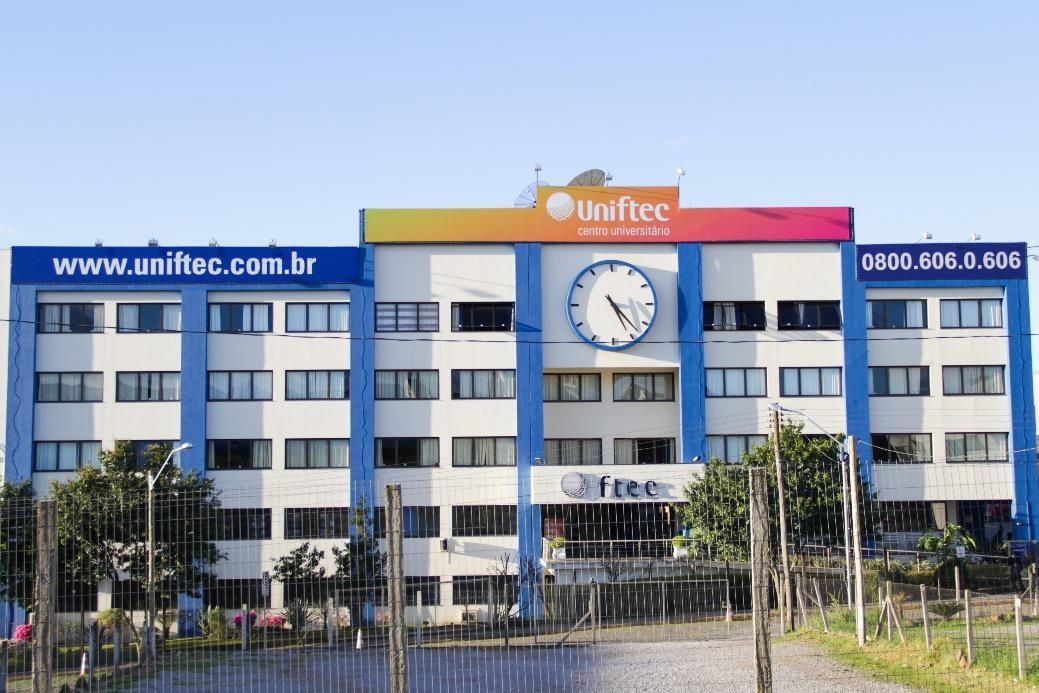
\includegraphics[width=1\textwidth]{img/fachada.jpg}
    \captionsetup{justification=normal}
    \legend{Fonte: Uniftec (2018)}
\end{figure}

\section{Assunto 2}

\lipsum[2-3]

\subsection{Sub assunto}

\lipsum[3-4]

\subsubsection{Sub-sub assunto}

\lipsum[4-5]

\subsubsubsection{Sub-sub-sub assunto}

\lipsum[5-6]

\chapter{Procedimentos metodológicos}

O \citeonline{ftec18} cita que, os procedimentos metodológicos consistem em descrever o seguinte:

\begin{enumerate}[label=\alph*)]
    \item a metodologia utilizada na realização da pesquisa;
    \item a população e/ou objeto investigado; bem como a amostragem;
    \item os procedimentos técnicos empregados na obtenção dos dados, como foram
construídos e utilizados;
    \item a explicitação dos tipos de fontes utilizadas e dados foram coletados; e e) o relato dos diferentes momentos do processo investigativo.
\end{enumerate}

O referido manual, também ressalta que deve ser utilizado o tempo verbal no passado.


\chapter{Apresentação e análise dos resultados}